\documentclass[10pt]{llncs}
\pagestyle{plain}

\usepackage[cmex10]{amsmath}
\usepackage{amssymb}
\usepackage{array}
\usepackage{bm}
\usepackage{graphicx}
\usepackage{epstopdf}
\usepackage[hang]{subfigure}
\usepackage{import}
\usepackage{booktabs}
\usepackage{tabularx}

\usepackage[colorlinks=true,linkcolor=blue,citecolor=blue,urlcolor=black]{hyperref}
\usepackage{algorithm, algpseudocode}

% Commenting functionality
\usepackage{todonotes}
%\reversemarginpar

\newcommand{\brs}[1]{\left[{#1}\right]} %square bracets
\newcommand{\brr}[1]{{\left({#1}\right)}} %round bracets
\newcommand{\brf}[1]{\left\lbrace{#1}\right\rbrace} %figure bracets
\newcommand{\brabs}[1]{\left\vert{#1}\right\vert} %absolute bracets
\newcommand{\norm}[2]{\left\|{#1}\right\|_{#2}} %norm_*

\newcommand{\I}[1]{\ensuremath{I\!\left[{#1}\right]}} %Robustness criterion I[*]
\newcommand{\Iq}[1]{\ensuremath{I_q\!\left[{#1}\right]}} %Robustness criterion I_q[*]
\newcommand{\Ic}[1]{\ensuremath{I_c\!\left[{#1}\right]}} %Robustness criterion I_c[*]

\newcommand{\vx}{\ensuremath{\mathbf{x}}} % vector x
\newcommand{\vX}{\ensuremath{\mathbf{X}}} % vector X
\newcommand{\vf}{\ensuremath{\mathbf{f}}} % vector f
\newcommand{\vz}{\ensuremath{\mathbf{z}}} % vector z
\newcommand{\vZ}{\ensuremath{\mathbf{Z}}} % vector Z
\newcommand{\vw}{\ensuremath{\mathbf{w}}} % vector w
\newcommand{\vd}{\ensuremath{\mathbf{d}}} % vector d
\newcommand{\vp}{\ensuremath{\mathbf{p}}} % vector p
\newcommand{\vP}{\ensuremath{\mathbf{P}}} % vector P
\newcommand{\vu}{\ensuremath{\mathbf{u}}} % vector u
\newcommand{\vU}{\ensuremath{\mathbf{U}}} % vector U
\newcommand{\DSet}{\ensuremath{\mathcal{D}}} % Set D
\newcommand{\NSet}{\ensuremath{\mathcal{N}}} % Set N
\newcommand{\XSet}{\ensuremath{\mathcal{X}}} % set X
\newcommand{\ZSet}{\ensuremath{\mathcal{Z}}} % set Z
\newcommand{\SSet}{\ensuremath{\mathcal{S}}} % set S
\newcommand{\Pref}{\ensuremath{\mathcal{P}}} % Preferences set P

\DeclareMathOperator*{\argmin}{\arg\!\min}
\DeclareMathOperator*{\argmax}{\arg\!\max}


\begin{document}
\title{sParEGO -- A Hybrid Optimization Algorithm for Expensive Uncertain Many-Objective Optimization Problems}
\author{Robin C. Purshouse\inst{1} \and Shaul Salomon\inst{2} \and Daniel C. Oara\inst{1} \and Peter J. Fleming\inst{1}}
\institute{Department of Automatic Control and Systems Engineering\\ University of Sheffield\\ Mappin Street, Sheffield S1 3JD, UK\\ \email{\{r.purshouse,dcoara1,p.fleming\}@sheffield.ac.uk}
\and Department of Mechanical Engineering\\ ORT Braude College of Engineering, Karmiel, Israel\\ \email{shaulsal@braude.ac.il}}

\maketitle

\begin{abstract}
Abstract here
\end{abstract}

\section{sParEGO}
The main idea is that the uncertain distribution in objective space of every candidate solution is not quantified through Monte-Carlo sampling\footnote{or other uncertainty quantification methods such as polynomial Chaos}, but every solution is evaluated once, and the distribution is approximated based on the performance of nearby solutions.

The algorithm includes the following stages:
\begin{enumerate}
\item Initilisation of $n$ solutions:
	\begin{enumerate}
	\item \label{random} $n/4$ random or Latin hypercube
	\item \label{perturbation} $n/4$ perturbation of \ref{random}. This ensures that every solution has at least one neighbour.
	\item $n/2$ perturbation of a random set selected from \ref{random} and \ref{perturbation}. This makes some neighbourhoods more dense than others.
	\end{enumerate}
\item Generate a set of direction vectors - Simplex Lattice
\item Evaluation
\item \label{direction} Select a direction. At every cycle, iterate over the entire set in a random order.
\item Scalarisation - General decomposition using weighted $Lp$ function.
\item Approximation of the univariate distribution for the scalar function value. Calculate the central tendency and variance according to the neighbourhood, and fit a normal distribution (standard error?)
\item Assign fitness according to a robustness criterion
\item Fit a Kriging model to the fitness
\item Optimize the maximum likelihood for improvement according to the model and its error
\item Evaluate the optimum solution and a perturbation of it, add them to the population and return to \ref{direction}
\end{enumerate}

\subsection{Parameters}
\begin{itemize}
\item $\delta$ -- Neighbourhood distance.
Maximum Euclidean distance between solutions in normalised decision space to be considered as neighbours.
Default value is $0.1 \sqrt{n_x}$.
\item $n_\text{init}$ -- Size of initial population.
\item $n_\text{indp}$ -- Portion solutions in the initial population that are independently generated.
Must be smaller or equal to $n_\text{init}/2$.
\item $\delta_\text{pert}$ -- maximum distance between newly generated solutions.
Default value is $\delta / 2$.
\item $n_d$ -- Number of sub-problems for decomposition (number of reference direction vectors).
\item Scalarisation function. The norm $p$ when using weighted $Lp$ scalarisation.
\item $c$ -- Desired level of confidence in the performance of the solutions.
\item $\alpha$ -- Level of confidence in parameters of the sampled distribution. Default is $c$.
\item $\beta$ -- Bandwidth of the Kriging model. Defines the intensity of spatial correlation between solutions in the model. Default is $0.1 \delta$.
\item $n_\text{max}$ -- Maximum number of solutions to construct the Kriging model.
\end{itemize}

\subsection{Initialisation}
To provide good initial coverage of potential designs, a space filling design (Latin hypercube) is used for the initial set.
However, the algorithm requires all solutions to reside within a distance of $\delta$ from other solutions (at least one).
To accomplish this, only $n_\text{indp} \leq n_\text{init}/2$ solutions are generated by Latin hypercube.
The rest of the solutions are generated as follows:
\begin{enumerate}
\item For every existing solution, another solution is randomly generated within a hypersphere with a radius of $\delta_\text{pert}$.
\item The rest of the solutions are generated by randomly selecting an existing solution and creating a nearby solution within a distance of $\delta_\text{pert}$.
\end{enumerate}
The first stage enforces that every solution has at least one neighbour.
The second stage seeds the initial population with neighbourhoods of different sizes.

\section{A decomposition-based approach to multiobjective optimization}
\label{sec:Decomposition}
Without loss of generality, consider the following unconstrained multiobjective optimization problem (MOP):
\begin{align}
\label{eq:mop}
	\min_{\vx\in\Omega} \vz=\vf\brr{\vx},
\end{align}
where \vx\ is a vector of $n_x$ decision variables in a feasible domain $\Omega$, \vz\ is a vector of $n_z$ performance criteria and \vf\ is a set of functions mapping from decision-space to objective-space:
\begin{align}
	\vf: \mathbb{R}^{n_x} \rightarrow \mathbb{R}^{n_z}
\end{align}
If some of the objectives are in conflict with one another, the solution to~\eqref{eq:mop} is expected to be a set of decision vectors, offering different trade-offs between the objectives.

\subsection{Normalisation} 
\label{subsec:Normalisation}
The decision variables and objectives are likely to be incommensurable, and therefore both decision-space and objective-space are normalised to non-dimensional units in the following manner:

\begin{align}
	\tilde{x}_i &= \frac{x_i - x^l_i}{x^u_i - x^l_i} , &i=1,\ldots,n_x,\\
	\tilde{z}_j &= \frac{z_j - z^*_j}{z^n_j - z^*_j} , &j=1,\ldots,n_z,
\end{align}
where $x^u_i$ and $x^l_i$ are the upper and lower boundaries of the $i^\text{th}$ decision variable, $z^n_j$ and $z^*_j$ are the $j^\text{th}$ components of the known nadir and ideal vectors\footnote{The ideal vector is composed of the best value of each objective. The nadir vector is composed of the worst value of each objective amongst all Pareto optimal solutions. Both vectors are estimated according to the current available information concerning the objective-space.}, and the tilde accent represents a normalised, dimensionless variable.

The normalised values are used for all operations within the algorithm. Before a candidate design is evaluated, it is re-scaled to the natural dimensions.

\subsection{Scalarising functions}
\label{subsec:Scalarising}
Over the last decade, decomposition-based evolutionary methods have gained increasing popularity for solving multiobjective optimization problems~\cite{Giagkiozis2013Overview}. A decomposition-based algorithm decomposes the MOP~\eqref{eq:mop} into $n$ single-objective problems, each targeting different ratios between the objectives. This sort of decomposition can be seen in Figure~\ref{fig:decomposition}: a set of six reference objective vectors is being used to guide the search towards different regions on the Pareto front. A different sub-problem is defined for every direction vector by using a scalarising function $f\brr{\vz,\vw}$ that maps an objective vector \vz\ into a scalar value according to a vector of weights \vw. The weights vector \vw\ is composed of non-negative components that sum to one.
The $i^\text{th}$ component of \vw\ is the relative weight of objective $z_i$.

\begin{figure}
	\centering
	\def\svgwidth{0.4\textwidth}
	\import{figures/}{decomposition.pdf_tex}
	\caption{Decompostion of a bi-objective problem into six single-objective problems, each aiming at a different ratio between the objectives.
	Reference direction vectors are marked in grey and corresponding Pareto optimal solutions in black.}
	\label{fig:decomposition}
\end{figure}

The scalarising function used in this framework is the popular \emph{weighted $L_p$}~\cite{koski1987norm,Marler2004Survey}:
\begin{align}
\label{eq:weighted Lp}
	s = \brr{\sum_{i=1}^{n_z} \brr{w_i\cdot \brr{z_i-z_i^*}}^p}^{1/p},
\end{align}
where $\mathbf{z^*}$ is a reference vector in objective space, typically the \emph{ideal} vector, which is composed of the minima of each individual objective. For a given weighting vector $\vw$, a comparison between two vectors $\vz^{A}$ and $\vz^{B}$ depends on the choice of norm $p$. Figure~\ref{fig:weightedLp} depicts the effect of using different values of $p$ for a bi-objective problem. The black point represent a desired ratio between the two objectives $\brs{0.3,0.7}$, and the black line passing through this point denotes all the objective vectors with this ratio. The coloured lines represent contours of the scalarising function of Equation~\eqref{eq:weighted Lp}. It can be seen that as the norm increases, vectors closer to the black direction line have lower function values than other non-dominated vectors farther away from the line.
\begin{figure}% 3D graphical demonstration
\centering
\subfigure[$p=1$]{
\label{subfig:weightedLp p1}
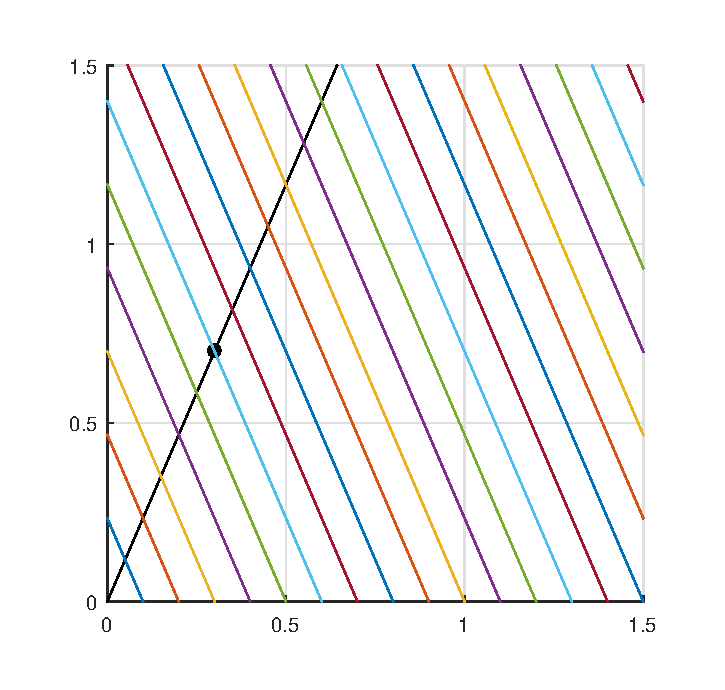
\includegraphics[width=0.31\textwidth]{figures/projectionContoursP1.eps}}
\subfigure[$p=3$]{
\label{subfig:weightedLp p3}
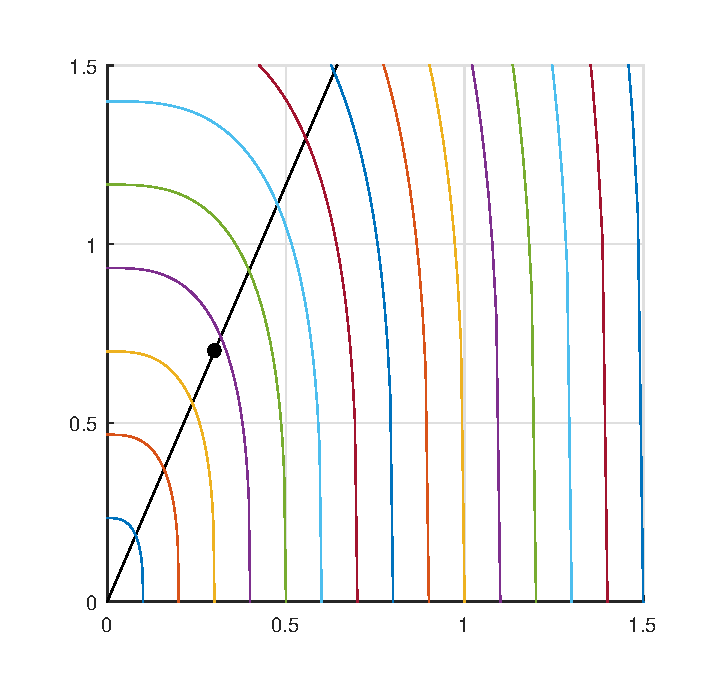
\includegraphics[width=0.31\textwidth]{figures/projectionContoursP3.eps}}
\subfigure[$p=50$]{
\label{subfig:weightedLp p50}
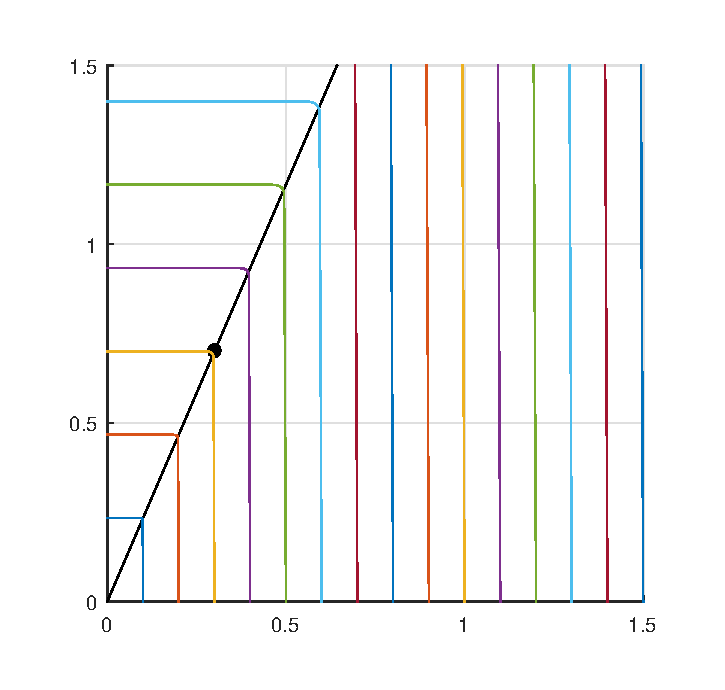
\includegraphics[width=0.31\textwidth]{figures/projectionContoursP50.eps}}
\caption{Contours of equal function values~\eqref{eq:weighted Lp} for different norms $p$}
\label{fig:weightedLp}
%% label for entire figure
\end{figure}

A high value of $p$ guarantees that the Pareto optimal solution that minimizes the scalarising function will possess the desired ratio between objectives. However, by using a higher norm the convergence of the algorithm becomes slower, since the focus is given to the single objective that has the largest deviation from the reference vector (as perhaps first noted in the literature in~\cite{borges1998basis}). In sParEGO, the weighted sum ($p=1$) is used in early stages to promote convergence, and the norm is gradually increased towards the final stages of the algorithm in an effort to find a well distributed set of solutions to present as possible trade-off choices.

For a given direction vector \vd\ there is a corresponding weighting vector that minimizes the scalarising function \cite{giagkiozis2014generalized}. The optimal weighting vector $\mathbf{w}$ for the scalarising function in~\eqref{eq:weighted Lp} is defined as:
\begin{align}
\begin{split}
	&\mathbf{w}=\brs{w_1,\ldots,w_{n_z}},\\
	&w_i=a\cdot\brr{d_i+\epsilon}^{-1} \quad , \quad i=1,\ldots,n_z,\\
	&\sum_{i=1}^{n_z} w_i=1,
\end{split}
\end{align}
where $\epsilon$ is a small number to prevent division by zero, and $a$ is a normalisation factor.

\subsection{Set of reference direction vectors}
\label{sec:Simplex Lattice}
The multiobjective optimization problem is decomposed to $n$ sub-problems as described in Section~\ref{subsec:Scalarising}. Each sub-problem $i$ correspond to a reference direction vector $\vd_i$ from a set $\DSet$. In the case where no preference information exists, the set is constructed using a Simplex Lattice design~\cite{Scheffe1958Experiments}:
\begin{align}
	\label{eq:SimplexLattice}
	\begin{split}
		\DSet = \Biggl\lbrace\vd=\brs{d_1,\ldots,d_{n_z}}\quad \vert \quad &\sum_{j=1}^{n_z} d_j = 1 \quad \wedge \\
		& \forall j, \quad d_j = \frac{l}{h}, l\in\brf{0,\ldots,h} \Biggr\rbrace.
	\end{split}
\end{align}
The number of direction vectors is determined by the dimensionality of the objective space, and the constant $h$: $\vert\DSet\vert = \binom{h+n_z-1}{n_z-1}$. The direction vectors are evenly distributed along the hyperplane $\sum z_j = 1$.

\section{Handling uncertainties}
\label{sec:Uncertainty Approximation}
The most important difference between sParEGO and ParEGO is that the former assumes that the outcome of an evaluation function is a realization of a random variate. Therefore, the scalarised function value cannot be used directly to construct the DACE model, and a utility indicator value is used instead. For every direction vector $\vd$, the surrogate model is constructed to search for a design that will optimize a given robustness indicator (described later in Section~\ref{sec:Robustness Indicators}). The guiding principle is to avoid Monte Carlo methods that repeatedly sample every candidate design to assess its statistical properties in objective-space. Instead, these properties (specifically, measures of central tendency and dispersion) are approximated from the available information of other candidate design evaluations.

The different sources of uncertainty, and the way they are propagated are described in Section~\ref{subsec:Uncertainty propagation}.
The steps for approximating the robustness indicator values of a set of candidate solutions are described in Section~\ref{subsec:Uncertainty quantification}. 

\subsection{Uncertainty quantification}
\label{subsec:Uncertainty quantification}
Sections~\ref{subsubsec:appx central}--\ref{subsubsec:robustness indicators} describe the methods for uncertainty quantification under a very limited budget of function evaluations. An illustration of the procedure is provided in Figure~\ref{fig:indicator_estimation}, and a summary is given in Algorithm~\ref{alg:Robust}.

In Sections~\ref{subsubsec:simple uncertainty quantification}--\ref{subsubsec:mixed complexity functions} describe the methods that can be used when some or all of the functions are not expensive to evaluate, and repeated evaluations are feasible.  

\subsubsection{Approximation of the central tendency}
\label{subsubsec:appx central}
Variations in decision-space are part of the problem description. This type of uncertainty is simulated by evaluating a sample of the random decision vector. For this reason, two designs with similar nominal values can be identical when realised. Therefore, the performance of a candidate design is calculated from the performance of neighbouring designs as well. A distance\footnote{Distance is measured in decision-space by the Euclidean norm.} in normalised decision space $\delta$ is defined, such that two solutions $\vx^i$ and $\vx^j$ are considered as neighbours if:
\begin{align}
	\norm{\vx^i-\vx^j}{2}\leq\delta.
\end{align}
For solutions in the set $\XSet$ that have neighbours, the statistical properties of their scalar fitness are approximated from the neighbouring solutions as follows:
First, the neighbourhood $\NSet^i$ of the design $\vx^i$ is defined\footnote{Note that according to~\eqref{eq:neighbourhood}, $\vx^i$ is included in the neighbourhood $\NSet^i$.}:
\begin{align}
	\label{eq:neighbourhood}
	\NSet^i=\brf{\vx^j\in \XSet \,\vert \,\norm{\vx^i-\vx^j}{2}\leq\delta}.
\end{align}
Next, the approximated mean function value is derived from the neighbourhood. Members that are closer to $\vx^i$ are given a larger weight in approximating its properties:
\begin{align}
	v^j &= \frac{\delta-\norm{\vx^i-\vx^j}{2}}{\delta}, \quad  \forall \vx^j\in\NSet^i,\\
\label{eq:neighbourhood mean}	\mu^i_s &= \left. \sum_{\vx^j\in\NSet^i} v^j s^j \middle/ \sum_{\vx^j\in\NSet^i} v^j \right. .
\end{align}

In Figure~\ref{subfig:indicator_estimation_a} the scalar fitness values of four candidate solutions (with a single decision variable) are depicted as grey dots. Solutions~$x^a,x^b,x^c$ are within a neighbourhood, while Solution~$x^d$ has no neighbours closer than $\delta$. The values of the expected mean $\mu_s\brr{x}$ are depicted as black dots.

\subsubsection{Approximation of the dispersion}
\label{subsubsec:appx dispersion}
Once the expected mean is known, the expected value for the variance is calculated:
\begin{align}
	\label{eq:neighbourhood variance}	\sigma^{2,i}_s = \left. \sum_{\vx^j\in\NSet^i} v^j \brr{s^j - \mu^i_s}^2 \middle/ \sum_{\vx^j\in\NSet^i} v^j \right. .
\end{align}
Since the variance in~\eqref{eq:neighbourhood variance} is calculated from a sample (possibly small), the standard error of the sample needs to be taken into account. This can be calculated from a chi-squared distribution with $\brabs{\NSet^i}-1$ degrees of freedom. For a confidence level $\alpha$ for the variance, the upper bound of the confidence interval is:
\begin{align}
	\label{eq:variance upper bound} \sigma^{\prime 2,i}_s = \frac{\sigma^{2,i}_s\brr{N-1}} {X^2_{1-\alpha/2}},
\end{align}
where $N=\brabs{\NSet^i}$ and $X^2_{1-\alpha/2}$ is the $1-\alpha/2$ percentile of a chi-squared distribution with $N-1$ degrees of freedom.

The intervals of $\mu_s\pm\sigma_s$ and $\mu_s\pm\sigma'_s$ are depicted in Figure~\ref{subfig:indicator_estimation_b} in red and blue, respectively.

\begin{figure}% 3D graphical demonstration
\centering
\subfigure[Estimation of the mean value (black) from the neighbourhood]{
	\label{subfig:indicator_estimation_a}
	\def\svgwidth{0.45\textwidth}
	\import{figures/}{indicator_estimation_a.pdf_tex}
}
\hspace{2mm}
\subfigure[Estimation of the variance (red) from the neighbourhood, and accounting for its standard error (blue)]{
	\label{subfig:indicator_estimation_b}
	\def\svgwidth{0.45\textwidth}
	\import{figures/}{indicator_estimation_b.pdf_tex}
}
\subfigure[Fitting of a Kriging model to existing $\sigma'_s\brr{x}$ (blue points). The blue line is the expected variance and the red lines represent the boundaries of the model error.]{
	\label{subfig:indicator_estimation_c}
	\def\svgwidth{0.45\textwidth}
	\import{figures/}{indicator_estimation_c.pdf_tex}
}
\hspace{2mm}
\subfigure[Assuming a normal distribution for $S$ according to $\mu_s,\sigma'_s$ for $x^a,x^b,x^c$, and  $s,\sigma''_s$ for $x^d$. The green area represents the indicator value $\Iq{x}$.]{
	\label{subfig:indicator_estimation_d}
	\def\svgwidth{0.45\textwidth}
	\import{figures/}{indicator_estimation_d.pdf_tex}
}
\caption{\subref{subfig:indicator_estimation_a}-\subref{subfig:indicator_estimation_c} Approximation of the statistical properties. \subref{subfig:indicator_estimation_d} Calculation of robustness indicator $\Iq{\bullet}$.}
\label{fig:indicator_estimation}
%% label for entire figure
\end{figure}

In order to approximate to properties of the distribution every candidate solution must have at least one neighbour.
To ensure that this is the case, whenever a new solution is added to the population, a near-by solution is generated by perturbing the new solution within its neighbouring proximity.

\subsubsection{Estimating the robustness indicator value}
\label{subsubsec:robustness indicators}
Once the mean and variance of the scalar fitness function have been estimated for every solution in the set, the random variable $S\brr{\vx}$ is assumed to follow a normal distribution. Given a desired threshold $q$ or a confidence level $c$,  the robustness indicator $\Iq{S}$ or $\Ic{S}$ can be calculated. An example for $\Iq{S}$ is given in Figure~\ref{subfig:indicator_estimation_d}.

\section{Threshold-based robustness metrics}
\label{sec:Robustness Indicators}
A general single-objective robust optimisation problem can be formulated as:
\begin{align}
\label{eq:rev:robust}
\min_{\vx\in\Omega} S=\vf\brr{\vx,\vU}.
\end{align}
Here, \vU\ is a vector of random variables that includes all the uncertainties associated with the optimisation problem. These uncertainties may be an outcome of manufacturing tolerances, a noisy environment, evaluation inaccuracies, and so on. A single scenario of the variate \vU\ is denoted as \vu. Since uncertainties are involved, the scalar objective $S$ is also a random variate, where every scenario of the uncertainties \vu\ is associated with an objective value $s$.

In a robust optimisation scheme, the random objective value is replaced with a robustness criterion, denoted by the indicator \I{Z}. Several criteria are commonly used in the literature, which can be broadly categorised into three main approaches:
\begin{enumerate}
%
\item \textbf{Worst-Case Scenario.} The worst objective vector, considering a bounded domain in the neighbourhood of the nominal values of the uncertain variables.
%
\item \textbf{Aggregated Value.} An integral measure of robustness that amalgamates the possible values of the uncertain variables (e.g. mean value or variance).
%
\item \textbf{Threshold Probability.} The probability for the objective function to be better than a defined threshold.
\end{enumerate}

In this framework the third approach, suggested by Beyer and Sendhof~\cite{Beyer2007}, is used. A threshold $q$ is considered as a satisfying performance for the objective value $s$. When $s$ is uncertain, denoted by the random variable $S$, the probability for $S$ to satisfy the threshold level can be seen as a confidence level $c$. For a minimization problem this can be written as:
\begin{align}
\label{eq:confidence}
	c\brr{S,q}=\text{Pr}\brr{S<q}.
\end{align}
Equation~\eqref{eq:confidence} can be used for two different robustness indicators:
\begin{enumerate}
	\item Minimization of the threshold $q$ for a pre-defined confidence level $c$, denoted as $\Iq{\bullet}$.
		This is useful when there is no specific target for performance, but the confidence in the resulting performance can be specified.
		The preferred solution is the one that guarantees the best performance with the specified confidence.
	\item Maximization of the confidence level $c$ for a given threshold $q$, denoted as $\Ic{\bullet}$.
		This measure can be used when the target for performance is known, and the emphasis is on meeting this target, rather than performing as well as possible.
\end{enumerate}

\section{sParEGO -- an algorithm for expensive, uncertain, many-objective optimization problems}
\label{sec:sParEGO}
The pseudo-code describing the complete sParEGO algorithm is given in Algorithm~\ref{alg:sParEGO}. Some comments about the stages are given below:
\begin{description}
	\item[Lines~\ref{line:randInit}-\ref{line:LHS} ---] To provide good coverage of potential designs, a space filling design (Latin hypercube) is used for half of the initial set. However, in the algorithm, it is also important to have neighbourhoods of solutions, and so the other half of the set is generated by small random walks from the space-filled design points.
	\item[Line~\ref{line:subset} ---] Above a certain size (approximately 100 solutions), the DACE model becomes prohibitively expensive to construct. When the number of evaluated solutions exceed this size, a subset is chosen according to the proximity of the direction of $\vz$ to the direction vector $\vd$.
	\item[Line~\ref{line:optimize model} ---] A single objective global optimization algorithm is used to maximize the expected improvement.
\end{description}

\begin{algorithm}
\caption{\textsc{sParEGO} pseudo-code}
\label{alg:sParEGO}
\begin{algorithmic}[1]
	\Statex \textbf{Parameters:} initial set size $n$, robustness criterion $I$,
	\Statex \hspace{22mm} evaluation functions $\vf$, neighbourhood distance $\delta$,
	\Statex \hspace{22mm} number of reference vectors $n_\text{max}$
	\State $\XSet \leftarrow$ initialise a random set of solution of size $n/2$
	\label{line:randInit}
	\State $\XSet \leftarrow \XSet \cup \textsc{LatinHypercube}\brr{\Omega,n/2}$ \Comment{Line~\ref{state:latin}}
	\label{line:LHS}
	\State $\ZSet \leftarrow \vf\brr{\XSet}$ \Comment{evaluate the initial set}
	\ForAll{$\vx^i\in\XSet$}
		\State calculate $\NSet^i$ \Comment{Equation~\ref{eq:neighbourhood}}
	\EndFor
	\While{stopping criteria not satisfied}	
		\State $\Pref \leftarrow$ elicit preferences
		\State $\DSet \leftarrow$ \textsc{SimplexLattice}($n_\text{max},\Pref$) \Comment{Algorithm~\ref{alg:SimplexLattice}}
		\State $p \leftarrow$ set the norm of scalarising function
		\ForAll{$\vd\in\DSet$}
			\State update ideal and nadir vectors
			\State choose a subset from $\ZSet$ according to \vd
			\label{line:subset}
			\State $\SSet \leftarrow$ calculate scalar fitness value \Comment{Section~\ref{subsec:Scalarising}}
			\State $Iset \leftarrow$ \textsc{RobustnessApproximation($\XSet,\SSet,\delta$)} \Comment{Algorithm~\ref{alg:Robust}}
			\State $model \leftarrow$ fit a DACE model to the indicator values $Iset$
			\State $\vx^\text{new} \leftarrow$ maximize the expected improvement based on $model$ \label{line:optimize model}
			\State $\XSet \leftarrow \XSet \cup \vx^\text{new}$
			\State $\ZSet \leftarrow \ZSet \cup \vf\brr{\vx^\text{new}}$ \Comment{evaluate the new solution}
		\EndFor
	\EndWhile
	\State \Return set of non-dominated solutions $\hat{\vx}$
\Statex
\Procedure{LatinHypercube}{$\Omega,n$} \label{state:latin}
	\State divide every dimension in $\Omega$ to $n$ equal intervals.
	\State \Return $n$ vectors such that every row is used by only one vector
\EndProcedure
\end{algorithmic}
\end{algorithm}

\section{Other aspects of the framework}
\label{sec:Other aspects}
\subsection{Attitude to risk}
\label{subsec:risk}
In robust design optimization, there is an inherent trade-off between the solution's expected performance and the confidence in achieving it under extreme scenarios of the uncertainties involved. sParEGO provides four parameters to express the decision maker attitude to risk:
\begin{itemize}
	\item When the robustness metric $\Iq{\bullet}$ is used, the confidence level $c$ can be specified.
	\item When estimating the variance upper bound $\sigma^{\prime 2}_s$  in Equation~\eqref{eq:variance upper bound}, the confidence level $\alpha$ can be specified.
	\item The value used for approximating the variance of isolated solutions $\sigma^{\prime\prime 2}_s$ in Figure~\ref{subfig:indicator_estimation_c}, represents a risk averse attitude. A less conservative approach would be not to consider a smaller value than the upper bound of the model prediction interval.
	\item The value $\delta$--the maximum distance between solutions to be considered as neighbours--affects the variance of solutions and the convergence rate.
		For smooth and continuous functions, a tight neighbourhood is likely to result in smaller variance, but also uses less information from other solutions, which reduces convergence rate.
\end{itemize}

\subsection{Convergence}
\label{subsec:convergence}
A convergence indicator for the current set of candidate solutions can be used by the decision maker to examine the progress of the search towards satisfying solutions. Two metrics are proposed, one is based on the robustness indicator $\Ic{\bullet}$ (probability for satisfying a specified target) and the other on $\Iq{\bullet}$ (the value for a given confidence level). If preferences are given in terms of target vectors, the first metric is used. Otherwise, the second metric is used (with a default confidence level if a confidence level has not been specified).

Both metrics are calculated for a set of solutions $\hat{\XSet}$, termed here as the \textit{approximated robust Pareto set}. For a set of direction vectors $\DSet = \brf{\vd^1,\ldots,\vd^{n_d}}$, $\hat{\XSet}$ is the set of candidate solutions that optimize the indicator value for every direction. Formally:
\begin{align}
	\label{eq:Xc} \hat{\XSet}_c &= \brf{\vx^i\in \XSet \,\vert\, \vx^i = \argmin_{\vx\in\XSet} \Ic{S\brr{\vx,\vd^i},\vd^i} }, &i=1,\ldots,n_d&,\\ 
	\label{eq:Xq} \hat{\XSet}_q &= \brf{\vx^i\in \XSet \,\vert\, \vx^i = \argmax_{\vx\in\XSet} \Iq{S\brr{\vx,\vd^i},\vd^i} }, &i=1,\ldots,n_d&.
\end{align}

Sections~\ref{subsubsec:C_c} and~\ref{subsubsec:C_q} describe how to derive the convergence metrics, denoted as $C_c\brs{\hat{\XSet}_c}$ and $C_q\brs{\hat{\XSet}_q}$.

\subsubsection{Convergence in terms of goal achievement}
\label{subsubsec:C_c}
The convergence metric $C_c$ is the overall probability for satisfying the aspiration function $I_{c\brr{\vd}}\!\brs{S}$. This probability can be calculated by averaging the probabilities for satisfying the target in each direction $\vd^i$:
\begin{align}
	C_c\brs{\hat{\XSet}_c} = \frac{1}{n_d}  \sum_{\vx^i\in\hat{\XSet}_c} \Ic{S\brr{\vx^i,\vd^i},\vd^i}.
\end{align}
Figure~\ref{subfig:convergence_Cc} demonstrates how $C_c\brs{\hat{\XSet}_c}$ is calculated for a set of four direction vectors.

\subsubsection{Convergence in terms of confidence level}
\label{subsubsec:C_q}
First the threshold $q$ for every direction is converted back to the objective space, and the set of vectors $\hat{\ZSet}_q$ (black dots in Figure~\ref{subfig:convergence_Cq}) is used to evaluate the quality of the set $\hat{\XSet}_q$. This is achieved by calculating the hypervolume~\cite{zitzler1999multiobjective} of the set $\hat{\ZSet}_q$ with respect to a reference point $\vz^r$.\footnote{The anti-ideal vector, containing the known worst values for every objective, is used as the reference point $\vz^r$.}

\begin{figure}
\centering
\subfigure[Calculating the convergence metric $C_c\brs{\hat{\XSet}_c}$. For clarity, the threshold $q$ is kept constant for all directions. The metric value is the average of all green areas.]{
	\label{subfig:convergence_Cc}
	\def\svgwidth{0.45\textwidth}
	\import{figures/}{convergence_attainment.pdf_tex}
}
\hspace{2mm}
\subfigure[Calculating the convergence metric $C_q\brs{\hat{\XSet}_q}$. The metric value is the shaded area. For clarity, the confidence level $c$ is constant for all directions.]{
	\label{subfig:convergence_Cq}
	\def\svgwidth{0.45\textwidth}
	\import{figures/}{convergence_hv.pdf_tex}
}
\caption{Two convergence metrics for a set of four solutions of a bi-objective problem. Every solution is depicted as a probability function for the scalarised function value. The threshold $q$ is marked with black dots and the probability for satisfying this threshold is the green area.}
\label{fig:convergence}
\end{figure}

\subsection{Solution validation}
\label{subsec:validation}
The framework described in this document provides an estimate of the performance of a candidate design in terms of a random distribution. The accuracy of this estimate relies on several factors: the ability of the user to capture the inputs and models uncertainty correctly, the available resources for repeated evaluations and the correctness of the methods for uncertainty quantification presented above.

The following method allows the user to validate their assumptions, and to correct the assumptions that cause the greatest mismatch. It is worth mentioning that the suggested validation steps require a large budget of function evaluations and availability of experimental data.
An indicator to quantify the correctness of the assumptions is presented in Section~\ref{subsubsec:closeness-to-target}. The way this indicator can be used to isolate and tune the most influential assumptions is described in Section~\ref{subsubsec:sensitivity}.

\subsubsection{Closeness-to-target indicator}
\label{subsubsec:closeness-to-target}
Consider a candidate design $\vx$ is has been selected for validation. A direction vector $\vd$ is chosen, and $\Iq{\vx,\vd}$ is used as a robustness indicator with a confidence level $c$. A \textit{closeness-to-target} indicator is defined based on a comparison of the values of the robustness indicator, calculated using four methods:

\medskip\noindent
\begin{tabularx}{\textwidth}{lcX}
$I_\text{sp}$	& --- & the sParEGO algoritm;\\
$I_\text{mc}$	& --- & a Monte Carlo simulation of $\vx$ as described in Section~\ref{subsubsec:simple uncertainty quantification};\\
$I_\text{act}$	& --- & a set of high-fidelity evaluations of $\vx$ (e.g. a set of physical prototypes);\\
$I_\text{mix}$	& --- & a Monte Carlo simulation of $\vx$, but replacing input pdfs, where possible, with whatever input data has been captured for the high-fidelity evaluations.
\end{tabularx}

$I_\text{act}$ is used as a reference, since it is based on data that is more accurate than the data used during the simulations. The closeness-to-target measure $\Delta$ is defined as the difference between the indicator value from any method to $I_\text{act}$. For example, $\Delta_\text{mc} = \brabs{I_\text{mc}-i_\text{act}}$ provides an insight on the overall validity of the elicited uncertainties of the inputs and evaluation functions, together with the accuracy of the evaluation functions.

\subsubsection{Sensitivity analysis for uncertainty elicitation}
\label{subsubsec:sensitivity}
The value of $\Delta$ in isolation may not be very meaningful, but comparing two $\Delta$ values can aid in detecting the magnitude and direction of any wrongness in the assumptions.
Consider a reference measure $\Delta_\text{r} = \brabs{I_\text{mix}-I_\text{act}}$, where $I_\text{mix}$ is calculated by replacing all input distributions with the distributions of the experimental input data. Then a Monte Carlo simulation is conducted by sampling the input distributions and the model's uncertainty, as defined in Section~\ref{subsec:model fidelity}.

Now, the elicited uncertainty for the $j^\text{th}$ evaluation function (denoted $f_j$) can be examined by defining  $\Delta_{f_j} = \brabs{I_{\text{mix},f_j}-I_\text{act}}$, where $I_{\text{mix},f_j}$ is the same as $I_\text{mix}$, but the uncertainty for $f_j$ is changed. A sensitivity measure $\rho\brr{f_j}$ is defined:
\begin{align}
	\rho\brr{f_j} = \frac{\Delta_{f_j}}{\Delta_\text{r}}.
\end{align}
Values of $\rho\brr{f_j} < 1$ indicate that the new assumption is more accurate than the previous, and vice versa.

Similarly, the effect of every assumption on the input uncertainties can be examined: Let $I_{\text{mix},x_i}$ be the indicator value calculated by replacing the distribution for $X_i$ from the experimental data with the one used for simulations (elicited by the expert), and $\Delta_{x_i} = \brabs{I_{\text{mix},x_i}-I_\text{act}}$. The sensitivity measure $\rho\brr{x_i} = \Delta_{x_i} / \Delta_\text{r}$ provides an insight on the validity of the expert elicited uncertainty for $X_j$.
If the above validation procedure is conducted for all inputs and the values of $\rho$ are compared, the most impactful wrong assumptions can be identified.

The effects of the attitude to risk within the sParEGO algorithm can be examined in a similar manner by using $I_\text{sp}$ to calculate $\Delta_\text{sp} = \brabs{I_\text{sp}-I_\text{act}}$ and $\rho = \Delta_\text{sp} / \Delta_\text{r}$. Different parameter settings will change the closeness-to-target value, and hence these parameters can be tuned.


\section{Conclusion}
\label{sec:conclusion}

\subsection{Framework limitations and risks}
This section summarises the assumptions made within the framework described in this document, and the risks associated with these assumptions.
\begin{itemize}
	\item \emph{The landscape is well behaved (i.e., smooth, continuous).} The uncertainty distributions are approximated according to available information for other candidate solutions. The underlying assumption for approximating in this way is that similar solutions have similar performance. If the functions are highly ragged and discontinuous, the surrogate models cannot accurately predict their behaviour.
	\item \emph{The dimensionality is small to medium.} The search is conducted on a surrogate model fitted to the existing evaluated solutions. The DACE model used in this framework typically produces good estimates for problems with up to 20 design variables.
	\item \emph{The problem formulation is appropriately elicited.} The outcomes from any use of the framework can only be as good as the information provided to it. Methodologies for robustly eliciting the problem formulation lie outside the scope of the project.
\end{itemize}


\bibliographystyle{splncs}
\bibliography{sparegoReferences}

\end{document}